\chapter{Verwandte Arbeiten}
\label{chap:verwarbeiten}

\section{Bildsegmentierung}
\label{sec:segmentation}

\subsection{Unbeaufsichtigte Bildsegmentierung durch Backpropagation}
\label{ssec:kanezaki}
In seinem Paper \cite{kanezaki} stellt Asako Kanezaki einen Ansatz vor, Convolutional Neural Networks zur Bildsegmentierung zu nutzen. Die Besonderheit an diesem Ansatz ist allerdings, dass er nicht wie frühere Versuche CNNs zur Bildsegmentierung zu nutzen auf überwachtem Lernen basiert, sondern unüberwachtes Lernen nutzt.

Dieser Ansatz erstellt eine Mapping-Funktion $c_n=f(x_n)$, die jedem der $N$ $p$-dimensionalen Pixel mit dem Merkmalsvektor $\{x_n\in\mathbb{R}^p\}_{n=1}^N$ eines Eingabebildes ein Clusterlabel $c$ mit $\{c_n\in\mathbb{Z}\}_{n=1}^N$ zuordnet.

Während das Resultat das gleiche wie bei überwachtem Lernen ist, wird hier weder eine Ground Truth, noch ein vorher angelerntes Neuronales Netz benötigt.

Erreicht wird dieses Ziel durch einen iterativen Prozess, in welchem ein anfangs untrainiertes neuronales Netz eine Bildsegmentierung erzeugt, welche anschließend mithilfe einer im Vorhinein erstellten, konstanten Segmentierung optimiert wird. Diese Segmentierung wird in diesem Paper über den SLIC-Algorithmus\cite{slic} erzeugt. Dieser Algorithmus ist in \figurename~\ref{fig:Kan18_01} anschaulich dargestellt. 

\begin{figure}[h]
	\center{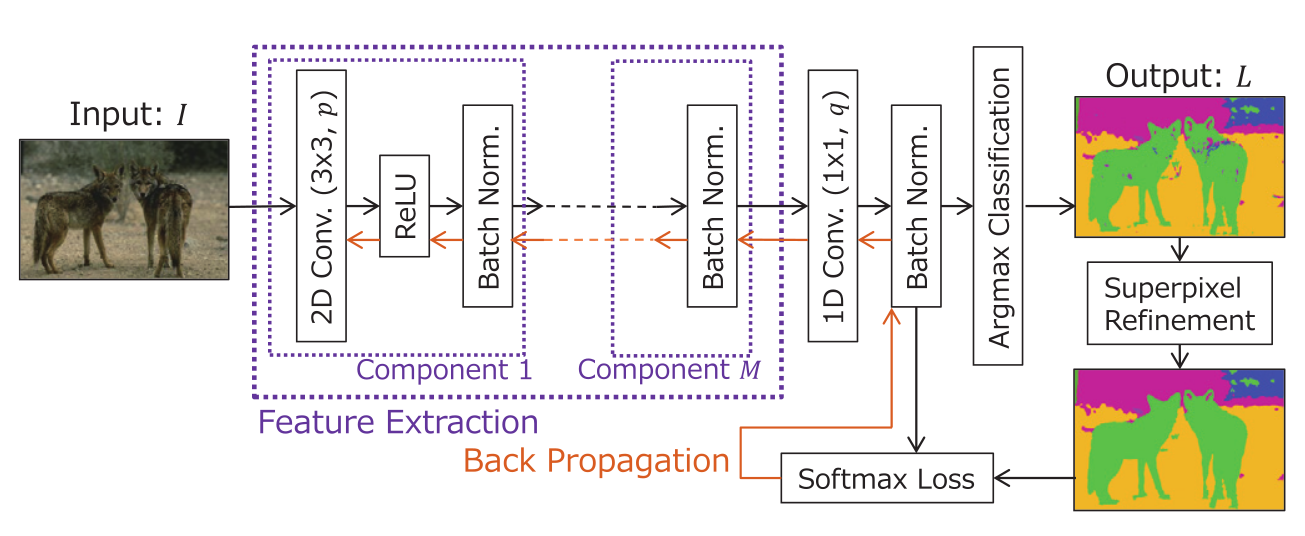
\includegraphics[width=.8\textwidth,keepaspectratio]{images/Kan18_01.png}}
	\caption{Vorgehensweise nach Kanezaki, aus \cite{kanezaki}}
	\label{fig:Kan18_01}
\end{figure}

%\section{Unsupervised Deep Embedding for Clustering Analysis}
%\label{sec:unsupervised_dec}
%\cite{unsupervised_dec}

\section{Kratererkennung}

\subsection{Automatisierte Kratererkennung}
\label{ssec:bandeira}
In dem Paper \enquote{Automatic Detection of Sub-km Craters Using Shape and Texture Information}\cite{bandeira} wird ein neuer Ansatz zur Kratererkennung vorgestellt. Zuvor wurden diese meist manuell katalogisiert, dies resultierte darin, dass nur die größten Krater dokumentiert wurden, oder darin, dass nur vergleichsweise kleine Bereiche innerhalb eines akzeptablen Zeitraums verarbeitet werden konnten. Daher konzentrieren sich die Autoren insbesondere auf die Erkennung von kleineren Kratern.

Die erarbeitete Vorgehensweise beginnt damit, dass über den Algorithmus von Urbach \& Stepinski\cite{urbach2009automatic} eine grobe Vorsortierung berechnet wird. Dieser Algorithmus ist zwar relativ effizient, hat aber nur eine Erkennungsrate von etwa 70\%. Er basiert auf der Tatsache, dass Krater meistens durch nebeneinander liegende Highlights und Schatten erkennbar sind.

Nach dieser Vorsortierung und den Pre-Processing Schritten (in Form von Histogramm-Optimierung) werden in \cite{bandeira} 9 Bitmasken (siehe \figurename~\ref{fig:BDS12_01}) in verschiedenen Positionen, Größen und Ausrichtungen über die Kandidaten gelegt. Die Wahrscheinlichkeit, dass der Kandidat ein Krater ist, berechnet sich aus der Übereinstimmung zwischen den Bitmasken und dem eigentlichen Kandidatenbild. Abschließend werden die Ergebnisse mithilfe eines angepassten AdaBoost Algorithmus optimiert. Das Post-Processing besteht aus der Eliminierung von ungewöhnlich geformten Kratern.

\begin{figure}[h]
	\center{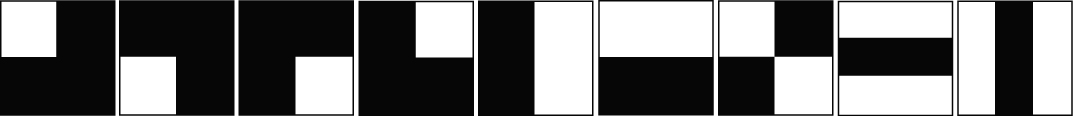
\includegraphics[width=.8\textwidth,keepaspectratio]{images/BDS12_01.png}}
	\caption{Die neun, zur Merkmalsextrahierung genutzen Bitmasken, aus \cite{bandeira}}
	\label{fig:BDS12_01}
\end{figure}

In \figurename~\ref{fig:BDS12_02} sind die von AdaBoost ausgewählten, am stärksten gewichteten Bitmasken-Überlagerungen dargestellt. Es ist zu beachten, dass der Krater im Hintergrund nur ein Beispiel ist, und nicht alle Krater, die von den jeweiligen Bitmasken überlagert werden, darstellt.

\begin{figure}[H]
	\center{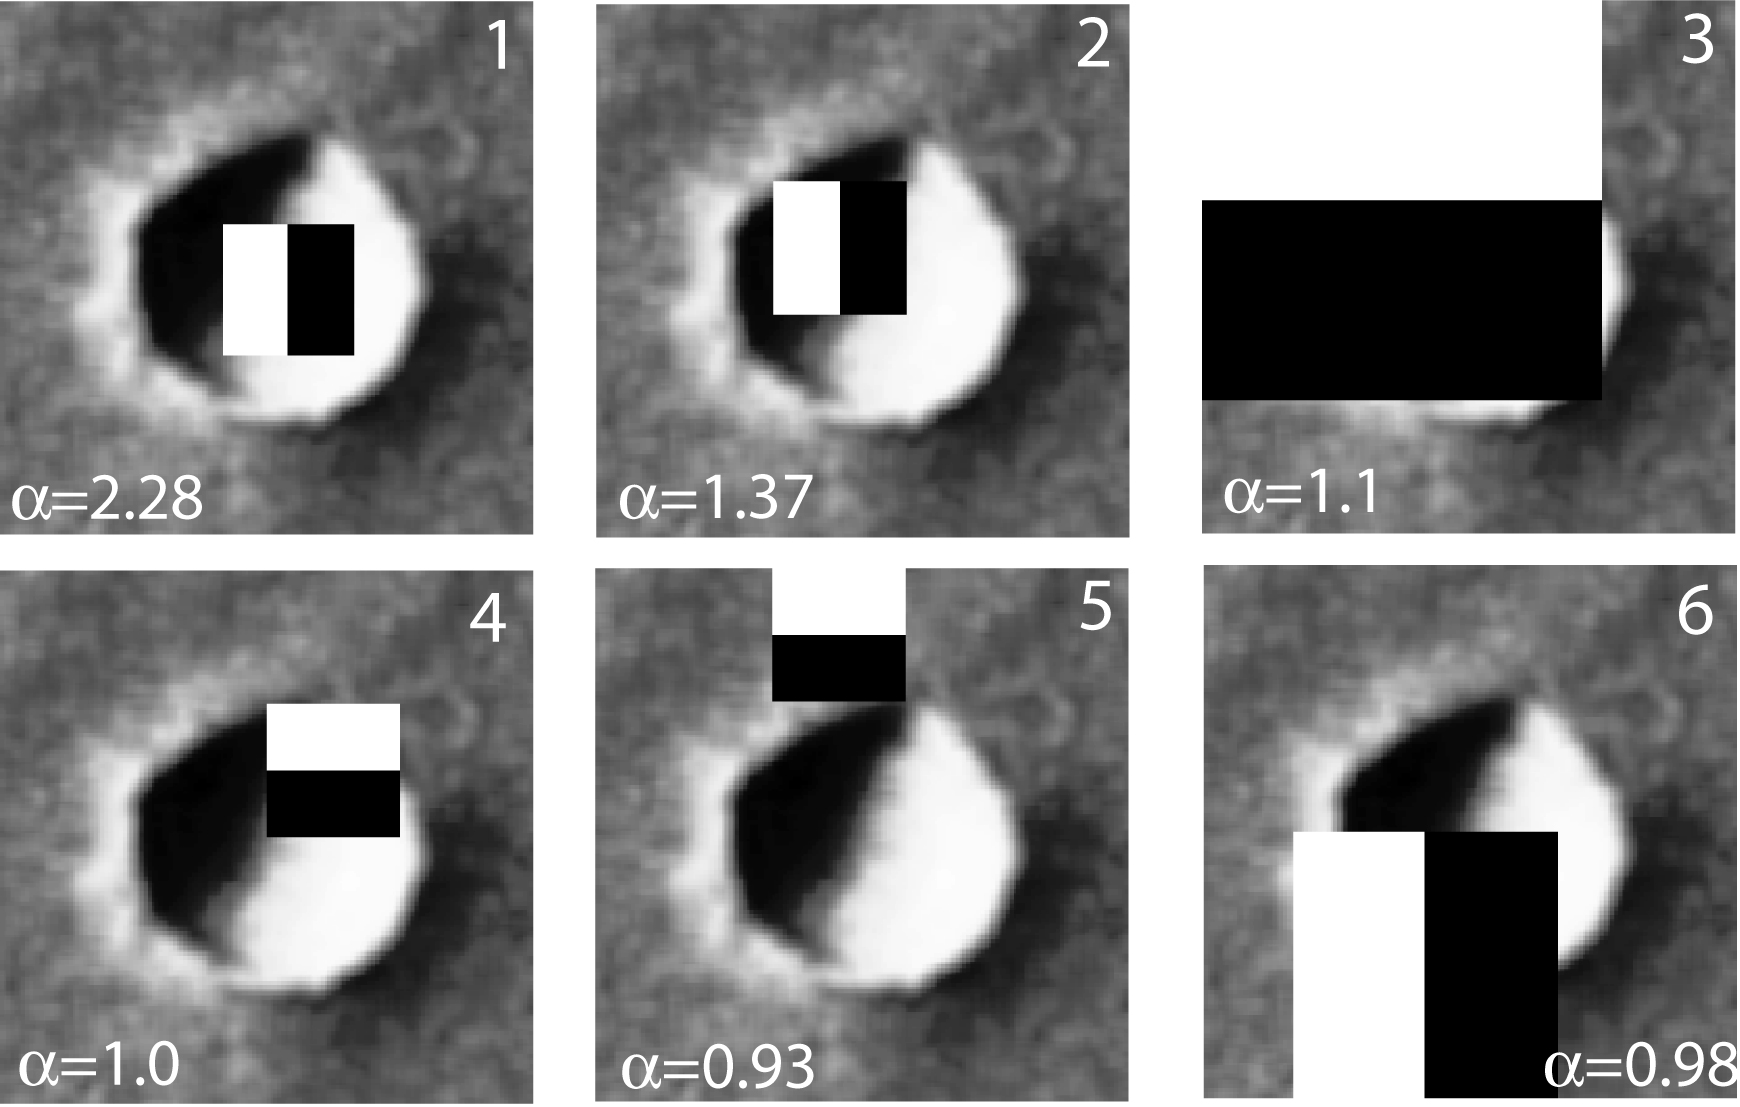
\includegraphics[width=.5\textwidth,keepaspectratio]{images/BDS12_02.png}}
	\caption{Die sechs am stärksten gewichteten Bitmasken, aus \cite{bandeira}}
	\label{fig:BDS12_02}
\end{figure}

Mit dieser Methode als Basis hat die \textit{University of Massachusetts Boston} einen Datensatz\cite{umass} erstellt, in dem eine Aufnahme des Mars von der HRSC\cite{neukum2004hrsc} auf Krater hin analysiert wird.


\subsection{Kratererkennung über Neuronale Netze}
\label{ssec:crater_cnn}
Auf der Basis des erwähnten, automatisch generierten Marskrater-Datensatz, wird in \cite{crater_cnn} ein neuronales Netzwerk daraufhin trainiert, selbst unterscheiden zu können, ob ein Kraterkandidat auch wirklich ein Krater ist. Die Architektur des Netzwerkes ist in \figurename~\ref{fig:CLLD16_01} zu sehen. Zur Evaluierung der Ergebnisse wird hier das 10-fache Kreuzvalidierungsverfahren genutzt. Dies bedeutet, dass der Eingabedatensatz zehn-geteilt wird, und jeweils neun Teile zum trainieren und ein Teil zum Evaluieren genutzt wird. Das Ergebnis ist der Durchschnitt der jeweiligen F1-Scores.% Es werden somit Werte von $88,78\%$, $88,81\%$ und $90,29\%$ für die drei jeweiligen Bereiche Westen, Mitte und Osten angegeben.

\begin{figure}[H]
	\center{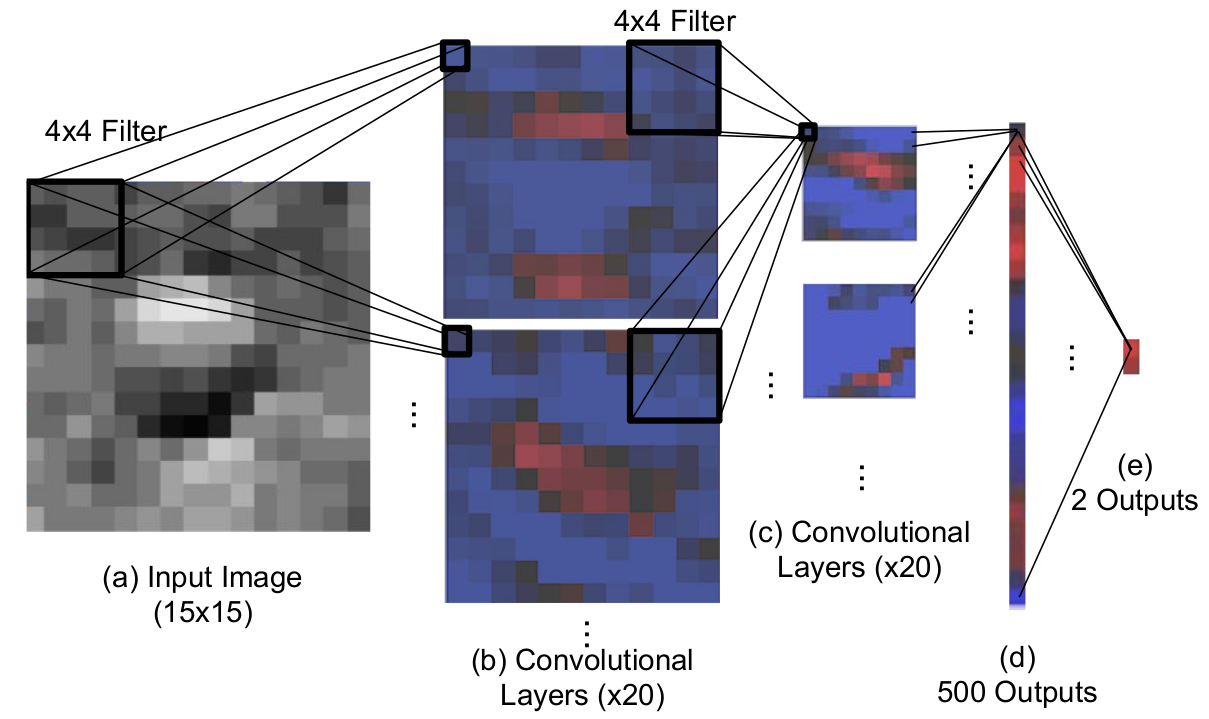
\includegraphics[width=.5\textwidth,keepaspectratio]{images/CLLD16_01.png}}
	\caption{Die Architektur des Netzwerkes, aus \cite{crater_cnn}}
	\label{fig:CLLD16_01}
\end{figure}

Der Unterschied zwischen dieser Methode und dem hier vorgestellten Ansatz besteht darin, dass in dieser Methode nur bewertet wird, ob Kraterkandidaten wirkliche Krater sind oder nicht, während hier ein Ansatz entwickelt wird, der aus einer kompletten Aufnahme der Marsoberfläche einzelne Krater(kandidaten) erkennt.

\subsection{Vergleich der Methoden}
\label{ssec:comparision}

In \tablename~\ref{tab:comparision} werden die vorgestellten Methoden zur Kratererkennung verglichen.

\begin{table}[h!]
\centering
\begin{tabular}{l | c c c}% TODO ÜBERPRÜFEN
	Region & Urbach '09 \cite{urbach2009automatic} & Bandeira '10 \cite{bandeira} & Cohen '16 \cite{crater_cnn}\\
	\hline
	Westen & $67,89\%$ & $85,33\%$ & $88,78\%$ \\
	Mitte & $69,62\%$ & $79,35\%$ & $88,81\%$ \\
	Osten & $79,77\%$ & $86,09\%$ & $90,29\%$ \\
\end{tabular}
\caption{F1-Scores der vorgestellten Methoden, adaptiert aus \cite{crater_cnn}}
\label{tab:comparision}
\end{table}